\documentclass[a4paper]{article}
\usepackage[francais]{babel}
\usepackage[utf8]{inputenc}
\usepackage[toc,page]{appendix} 
\usepackage[T1]{fontenc}
\usepackage{graphicx}
\usepackage{fancyhdr}
\usepackage{xcolor}
\usepackage[colorlinks=true,linkcolor=darkgray,urlcolor=blue,filecolor=blue]{hyperref}

\pagestyle{fancy}

% définir les entêtes et pieds de page
\lhead{Master Bioinformatique}
\rhead{Université Claude Bernard Lyon 1}
\renewcommand{\footrulewidth}{0.4pt}
\lfoot{UE Projet 2}
\rfoot{Février 2017}

% définir le titre et les auteurs sur la couverture
\title{{\sc \large Cahier des charges}\\
\bf Un site web interactif pour une meilleure compréhension de l’histoire évolutive des espèces}
\author{ShangNong {\sc Hu}\and Valentin {\sc Reymond}\and Grégoire {\sc Siekaniec}\and Krystian {\sc Valenducq}}
\date\today

% pour que la numérotation commence à partir de la deuxième page
\setcounter{page}{0}


\begin{document}

\begin{figure}[!t]
	\centering
	
\includegraphics[width=6cm]{./img/ucbl.png}
	\hspace{\fill}
	
\includegraphics[width=2cm]{./img/lbbe.png}
\end{figure}

\maketitle
% couverture sans numérotation
\thispagestyle{empty}

\begin{figure}[!b]
	\centering
	
\includegraphics[width=6cm]{./img/logo.png}
\end{figure}

\newpage

\tableofcontents
\newpage


\section{Contexte biologique}
	\paragraph{}
	La vie sur Terre est apparu il y a quelques milliards d'années. Il a fallut de nombreuses étapes pour que cette grande histoire parvienne jusqu'à l'Homme et ses espèces contemporaines. Cette histoire est parsemée de nombreuses péripéties qui ont résulté par l'apparition et la disparition de très nombreuses espèces. Ces variations sont dues à de nombreuses extinctions qui ont eu lieu au cours des temps géologiques. En revanche ces bouleversements dans l'histoire de la Vie restent à l'heure actuelle très floues quant à leur intensité et leur origine.

	\paragraph{}
	De nos jours, le grand public adopte une vision biaisée de l'évolution, tel qu'il existe qu'une seule extinction qui a été celle des dinosaures. Alors que d'après les connaissances actuelles, on peut recenser jusqu'à sept extinctions massives dont celle des dinosaures est la plus récente.
	% à verifier le nombre

	\begin{figure}[!h]
		\centering
		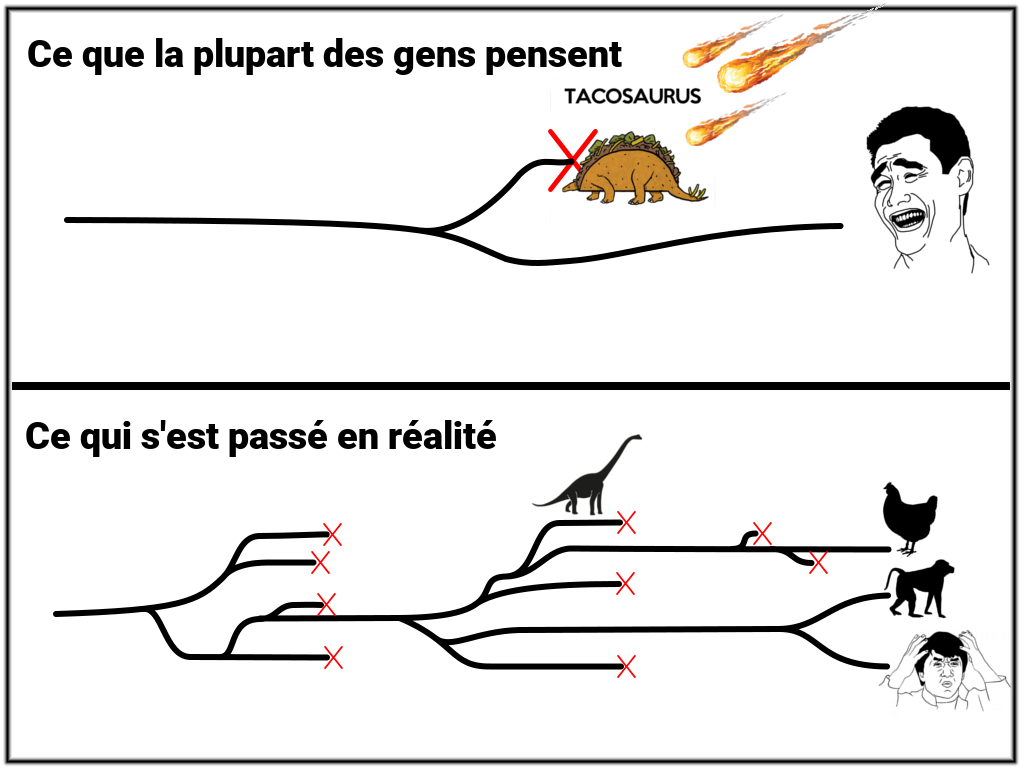
\includegraphics[width=12cm]{./img/illustr1.png}
		\caption{La vision biaisé face à la connaissance actuelle.}
		\label{comic1}
	\end{figure}

	\paragraph{}
	Les trois chercheurs de l'Équipe Bioinformatique, Phylogénie et Génomique Évolutive à LBBE (UCBL Lyon 1), D. M. de Vienne, J.-P. Flandrois et L. Guéguen se sont interessés à la sensibilisation de cette vision plus cohérente chez le grand public.

\section{Analyse des besoins}

	L'idée serait de retracer ces événements à l'aide d'un site web interactif, qui pourra par la suite être utilisé dans un but pédagogique (Université, Musée,\ldots).

	\subsection{Caractéristiques de la plateforme à mettre en place}
		\paragraph{}
		Le produit attendu sera un site web intéractif et responsive, c'est-à-dire accessible depuis différents appareils (Ordinateur, Tablette, Smartphone, \ldots).
		
		\paragraph{}
		Il sera chargé de présenter la \emph{timeline} de la vie, depuis l'apparition de la vie jusqu'à ce jour. Les événements de la vie seront présentés sous forme d'un arbre orienté horizontalement, et explorable depuis une barre de navigation.	De plus, cet outil permettra de mettre en lumière les différentes grandes crises qui ont eu un impact sur la densité des espèces au cours du temps. L'afficha mettra également l'accent sur les événements remarquables (tels que l'extinction des dinosaures). 
		
		\paragraph{}
		Nous souhaitons implémenter des informations supplémentaires concernant les taxons les plus représentatifs pour conserver un design intuitif et compréhensible.
		La navigation sera accompagnée d'une échelle de temps, afin que l'utilsiateur puisse se situer dans l'immensité des temps géologiques.
				

	\subsection{Outils utilisés pour répondre aux besoins}
		\paragraph{HTML5/CSS3}
		La page web sera créé en HTML/CSS, qui assurera l'affichage des éléments de base.
		Nous utiliserons W3.CSS pour la décoration par simplicité et expérience. Il nous permettra de rendre notre page web responsive. Il sera donc consultable sur la pluspart des appareils disponible.

		\paragraph{JavaScript}
		La partie interaction et animations de base sera réalisé par des script JS. Quant à l'affichage des données plus sophistiquées, nous aurons recours à D3.js.

		\paragraph{D3.js}
		Il s'agit d'un framework graphique créé à base de JavaScript, spécialisé dans l'affichage de données\footnote{\url{https://d3js.org/}}. Il nous permettra d'afficher l'arbre, la chronologie, ainsi que les diverses informations de manière interactive. 
		Ce framework inclu de multiples packages qui donnent lieu à des représentation graphiques très riches. 

		\paragraph{Python 2.7}
		Pour générer notre arbre nous avons recours à un algorithme de colonisation de l'espace. Cet algorithme est écrit en Python 2.7, car le module Matplotlib permettant l'affichage de l'arbre n'étant pas encore bien fonctionnelle sur la version 3 de Python. Il sera long de reprogrammer à partir du début, nous sommes donc rester sur ce script avec Python 2.7. 
	
	\subsection{Ordre de priorité}
		
		Il est important de définir un ordre de priorité dans la gestion des tâches pour la réalisation de ce projet. Nous disposons en effet d'un temps imparti relativement court.

		
		En première approche nous devrons élaborer un script pour générer un arbre qui soit le plus représentatif de l'histoire évolutive de la vie sur Terre. Cet arbre devra bien montrer l'existence des grandes extinctions. 
		En second lieu il faudra créer la monture de notre site, avec les différentes parties, notamment celle qui devra accueillir l'arbre.
		Une fois la structure du site terminé, nous devrons intégrer notre arbre avec des scripts javascript, notamment avec D3.js, pour obtenir les ramifications qui représenteront la biodiversité à un temps T. Cet arbre sera accompagné d'une échelle des temps géologiques, qui nous servira à nous situer dans l'histoire évolutive.

		
		Enfin, s'il nous reste du temps, nous pourrons peaufiner notre site en y ajoutant des options complémentaires, comme par exemple le taux d'oxygène présent lors d'une période particulière, ou encore les épisodes d'ères glaciaires. Ces informations complémentaires peuvent apporter une meilleure compréhension des évenements qui ont fait varier la densité de la biodiversité au cours du temps.

\section{Analyse de l'existant}
	Il existe sur internet des réalisations dont notre projet est inspiré. Nous avons également à disposition l'algorithme de M.DUCHEMIN qui permet de dessiner de manière réaliste des arbres en deux ou trois dimensions.

	\subsection{If the moon were only one pixel}
		L’idée de ce projet est de faire prendre conscience au grand public de l'immensité du vide qui nous entoure. Ainsi l'utilisateur se déplace dans le système solaire en scrollant horizontalement\footnote{\url{http://joshworth.com/dev/pixelspace/pixelspace_solarsystem.html}}. C'est en quelque sorte une carte du système solaire à l'échelle : diamètre de la lune = 1 pixel. Une échelle graduée nous accompagne lors de ce voyage dans l'espace afin d'accentuer la grandeur de ses distances. L'utilisateur s’aperçoit alors très vite que la majorité du système solaire est constitué de vide. Pour rendre l'expérience plus ludique, les développeurs ont eu la bonne idée de combler le vide par des petits messages informatifs, parfois à ton humoristique. Il nous est aussi possible de voyager à la vitesse de la lumière, on se rend alors compte que même à cette vitesse le voyage est très long.         
 		
	\subsection{TimeTree}
		Ce projet a pour objectif de représenter l'histoire de la Terre. Les 4,5 milliards d'années de son existence sont symbolisées par le tour d'une horloge\footnote{\url{http://deeptime.info/}}. On peut alors situer dessus les grandes ères géologiques, d'important événements géologiques (formation de la lune par exemple) ainsi que les groupes biologiques qui ont été importants dans l'évolution de la Vie. Le site est interactif, en cliquant sur le nom d'une ère par exemple, on est alors redirigé vers une information reliée.      
	
	\subsection{Onezoom}
		Ici le but de ce site web est d'illustrer l'arbre de la Vie depuis son apparition sur notre planète. Un arbre en forme de spirale représente la phylogénie de toutes les espèces\footnote{\url{http://www.onezoom.org/}}. On y voit alors les relations entre espèces et on prend conscience de la diversité biologique par la taille et le nombre de ramification de cette arbre. On peut se déplacer dans cette spirale en zoomant et cliquant sur les espèces qui nous intéresse pour avoir plus d'informations sur ces dernières.    	

	\subsection{Lifemap}
		Blablabla\footnote{\url{http://lifemap.univ-lyon1.fr/}}

	\subsection{Algorithme de colonisation de l'espace}
		Cet algorithme est un algorithme utilisé dans les jeux vidéos pour fabriquer un arbre réaliste de manière aléatoire. Dans notre cas, il nous est demandé de le modifier et de l’adapter à la création d’un arbre de la Vie démarrant  de l’origine de la vie et allant jusqu’à notre époque.
	
		Deux possibilité s’offre à nous :  recoder l’algorithme en partant du départ ou utiliser un algorithme déjà écrit par Wandrille Duchemin en le modifiant pour les besoins du projet, cet algorithme prend déjà en compte la possibilité d’ajouter des extinctions d’espèces à des moments indiqués dans le script :
		\begin{figure}[!h]
			\centering
			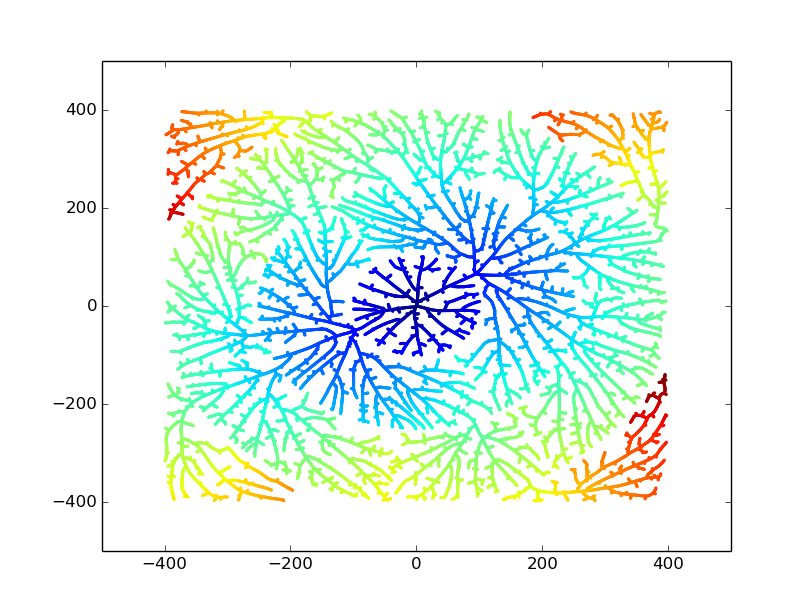
\includegraphics[width=12cm]{./img/multipleExtinction.png}
			\caption{Exemple d'arbre obtenu avec l'agorithme fourni}
		\end{figure}
	
		Le fonctionnement de l’algorithme de base est décrit dans le papier \emph{Modeling Trees with a Space Colonization Algorithm}\footnote{\url{http://algorithmicbotany.org/papers/colonization.egwnp2007.pdf}}, {Runions \emph{et al}, 2007.
	
		L’algorithme se déroule en différentes  phases :
		\begin{enumerate}
			\item Création d’une zone que l’on remplis avec des points d’attractions de manière aléatoire (par exemple un rectangle de 200 de largeur sur 1000 de longueur). 
			\item Positionnement de notre point arbre (branche) de départ (pour nous en x=0 et y =0).
			A ce moment on a quelque chose qui ressemble à cela :
			\begin{figure}[!h]
				\centering
				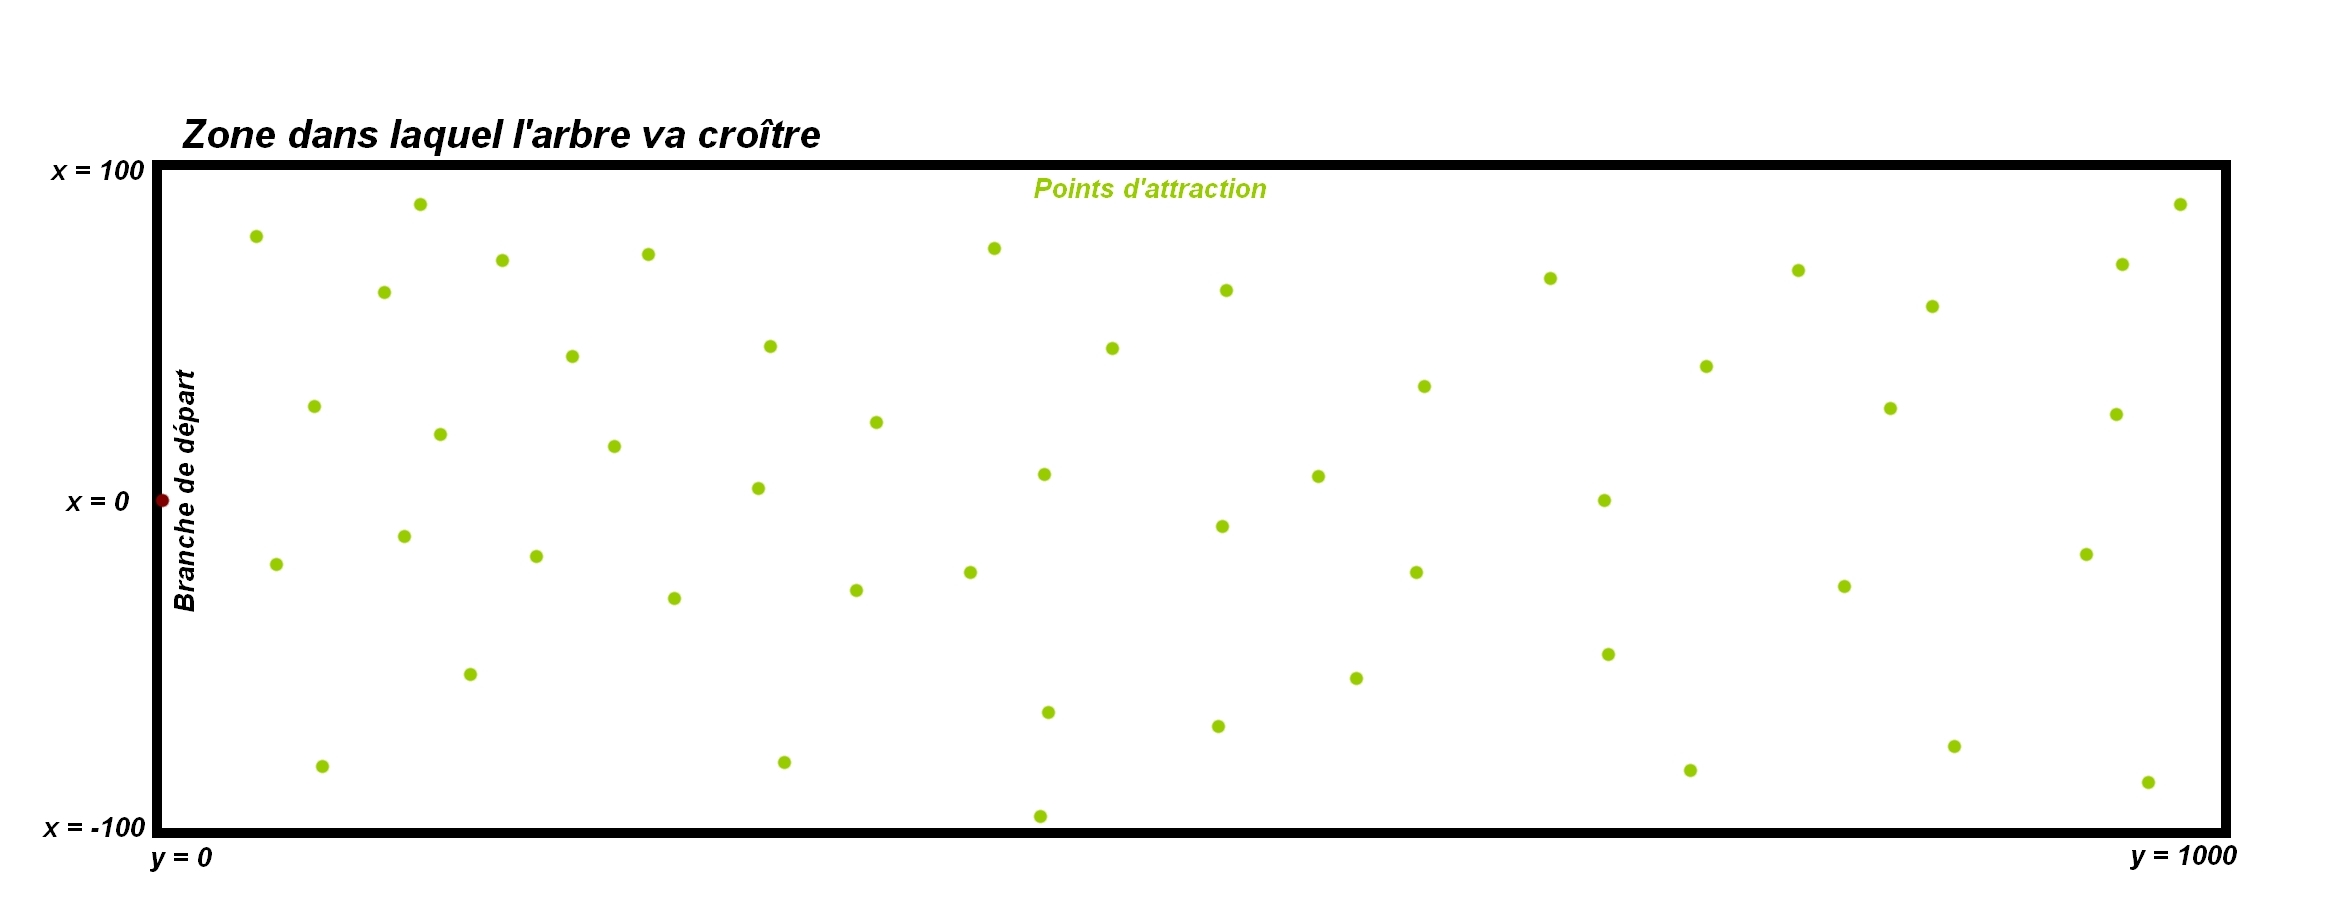
\includegraphics[width=11cm]{./img/sc.jpg}
				\caption{rien pour l'instant}
			\end{figure}
			\item Ensuite pour chaque point d’attraction on récupère la branche la plus proche présente dans son rayon d’attraction. Si cette branche est dans un « rayon minimum » par rapport au point d’attraction ce dernier devient inactif.

			\item On calcul alors un vecteur pour chaque branche en prenant en compte tout les points d’attractions de la manière suivante (chaque vecteur dépend des points d’attraction et du vecteur d’avant) et ont crée le nœud fils qui suit le vecteur : 
			\begin{figure}[!h]
				\centering
				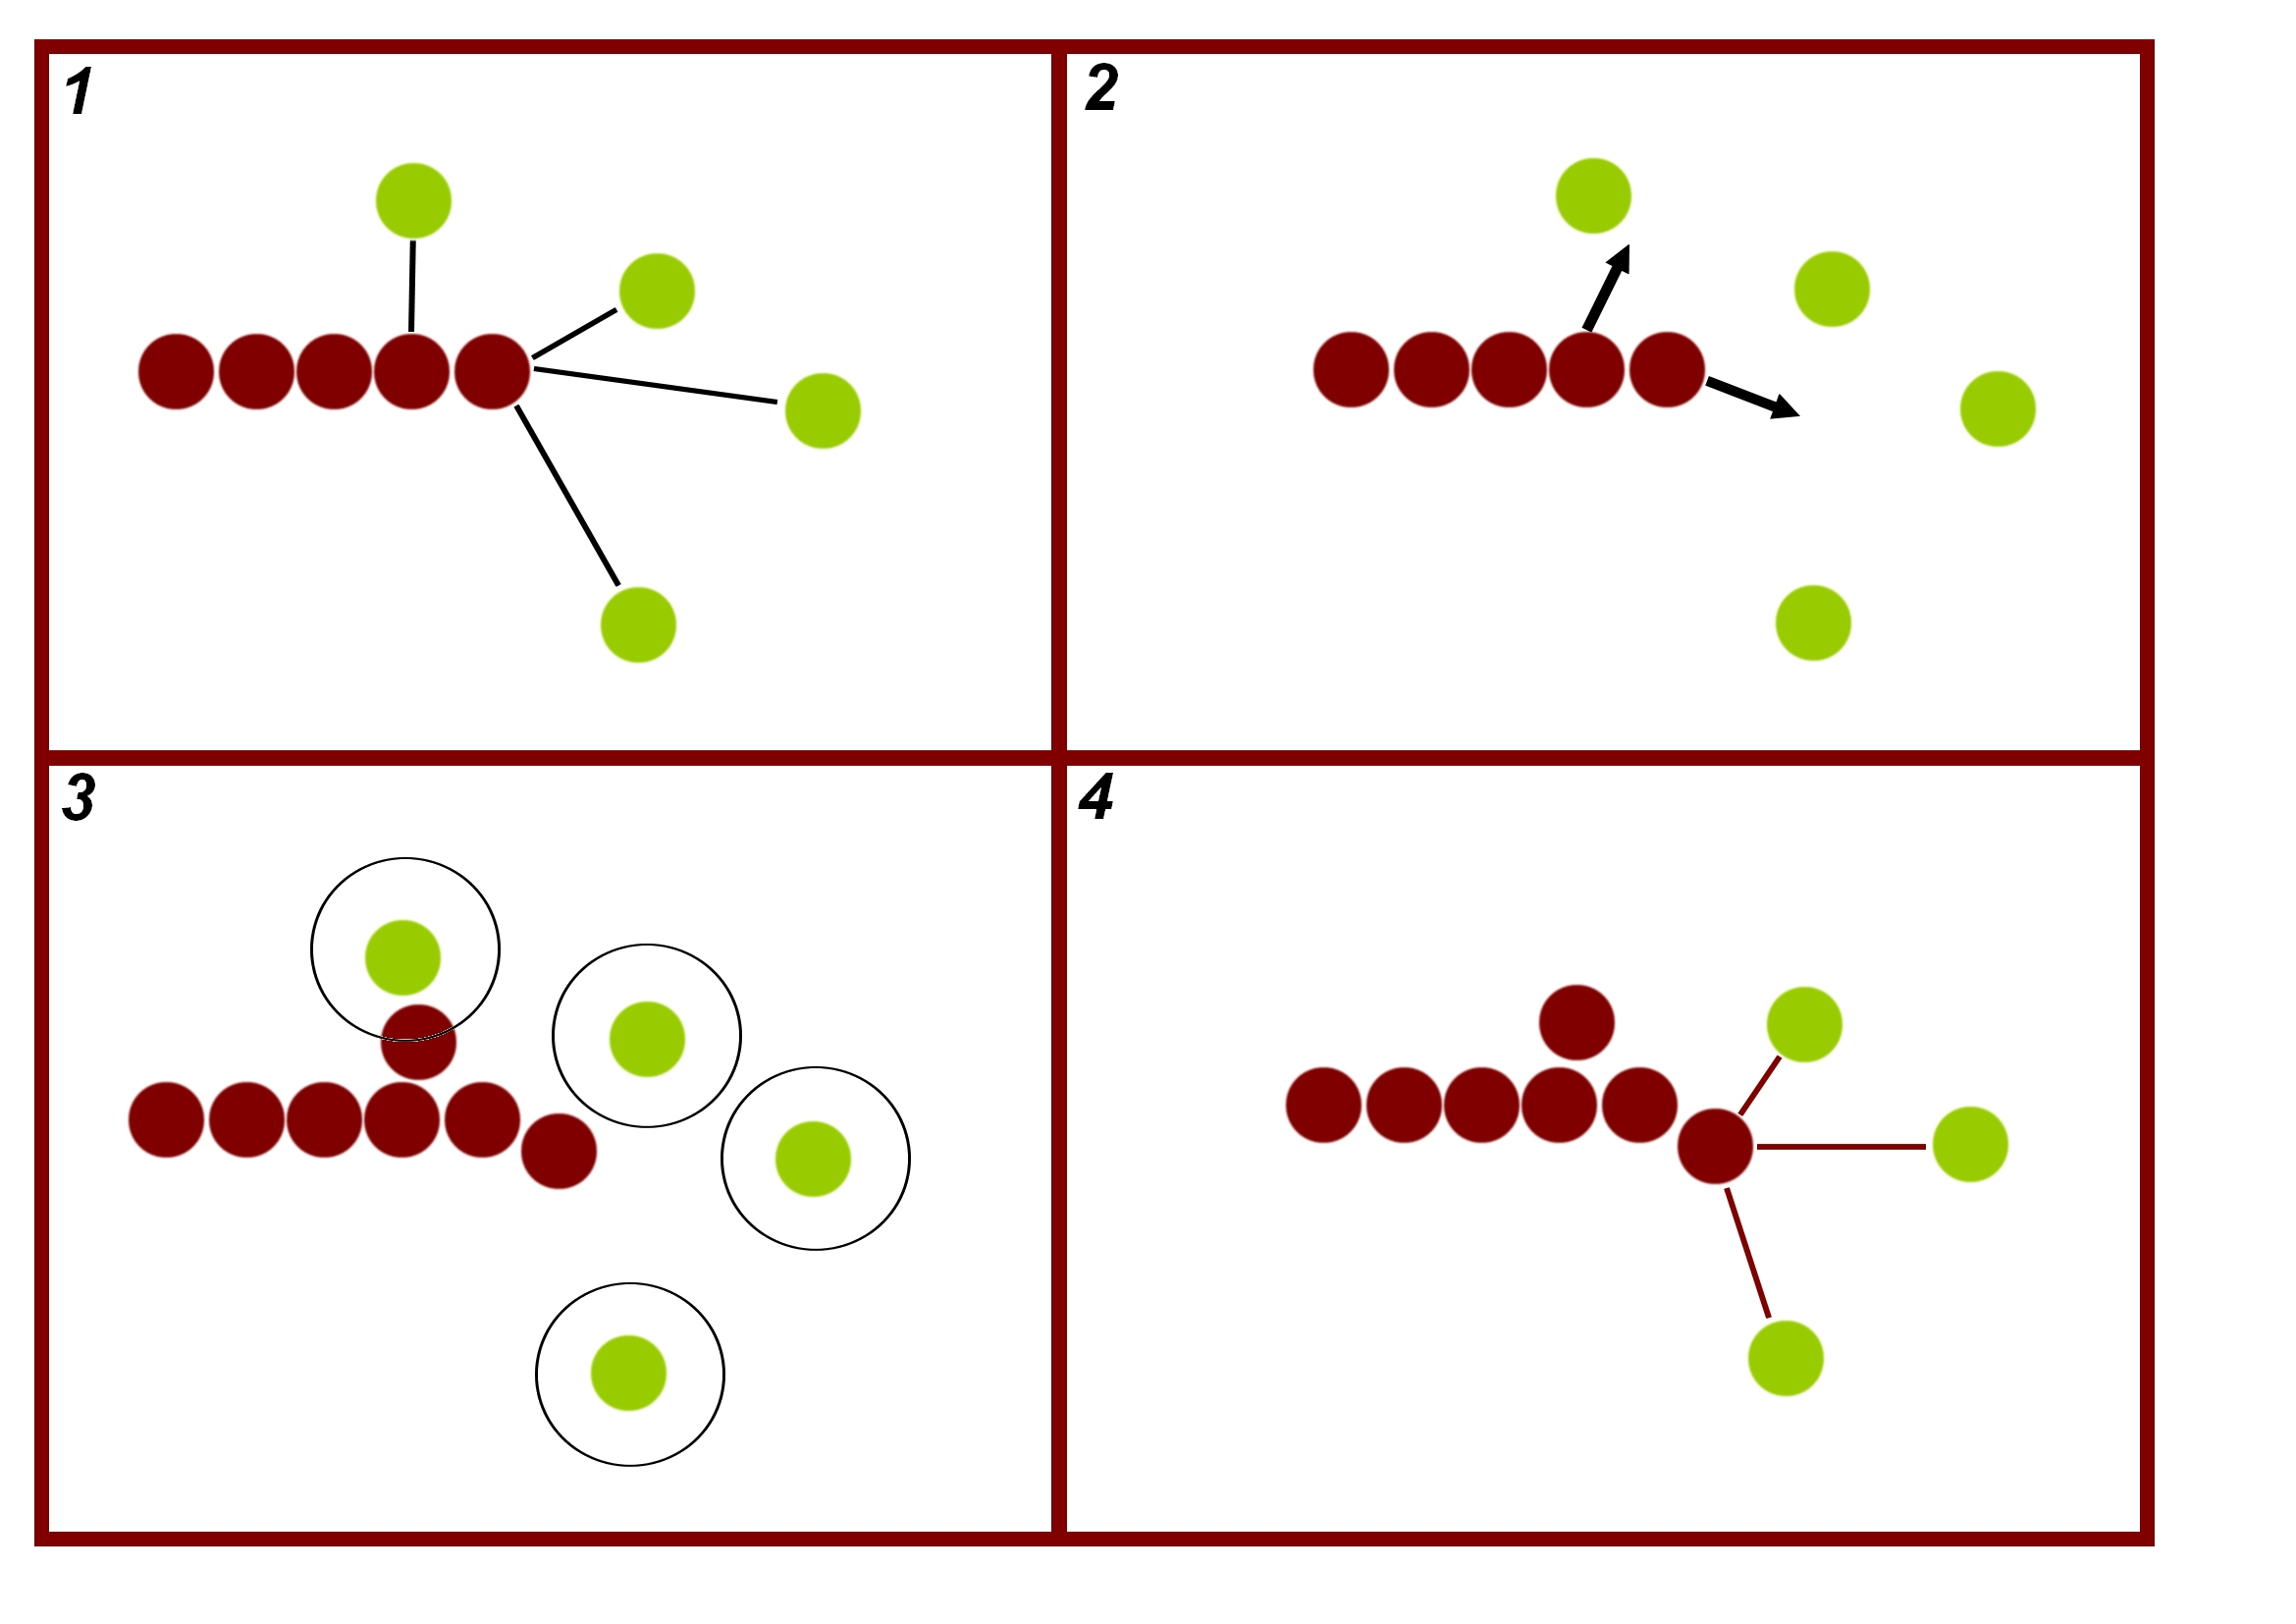
\includegraphics[width=7cm]{./img/sc2.jpg}
				\caption{rien pour l'instant}
			\end{figure}
			\item On fait cela en boucle jusqu’à ce qu’il n’y es plus de possibilité de croître ou que la boucle atteigne son maximum.
		\end{enumerate}


\section{Déroulement du projet}
	
			
	\subsection{Construction de la structure d'arbre}

			

	\subsection{Trouver les dates des évènements}

			

	\subsection{Afficher les données sur la page}
		

\section{Contraintes}

	\subsection{Contrainte temporelle}
		La date de rendu du cahier de charge est prévue le vendredi 17 février.
		La soutenance est prévue provisoirement le vendredi 24 mars, dont le délivrable devrait être rendu 2 jours avant.
		Le projet doit être développé dans une période de 1 mois.

	\subsection{Contraintes techniques}
		La principale contrainte technique résidera dans l'appréhension et la compréhension de l'algorithme de colonisation de l'espace. Il faudra pouvoir l'adapter à nos besoins, c'est-à-dire qu'il puisse s'ancrer correctement au sein de notre site. Nous devons également orienté le sens de son expansion, de la gauche vers la droite, pour qu'il puisse correspondre aux besoins attendus pour ce projet. Enfin, il devra bien marquer les grandes extinctions qui se sont déroulés lors des temps géologiques.

		D'autres contraintes peuvent apparaître, notamment lorsque nous devrons intégrer notre arbre sur notre site internet, il faudra alors bien trouver une concordance entre les différents codes que nous allons utiliser. De plus, nous devrons faire l'apprentissage de la riche bibliothèque Javascript qu'est D3.js.
		

	\subsection{Autres contraintes}

\section{Ouverture}

	Après avoir finalisé notre projet, nous pouvons nous projetter un petit plus loin de ce qui aura été fait. Ce travail fourni pourra servir de base à d'autres développeurs, ou encore pourra être mis en ligne pour en donner l'accès au public. Nous pouvons également penser à l'intégrer au sein de musée, afin d'apporter une touche ludique à l'Histoire de l'origine de la vie.
	De nombreuses otpions pourons être implémenter, cela peut aller à la description très précises d'espèces, et non pas s'arrèter au taxon. On peux aussi penser à rajouter des options supplémentaires, comme par exemple les fossiles connus, pour montrer jusqu'où nous sommes capable de remonter.


\section{Références}\label{Ref}
	\begin{enumerate}
		\item Adam Runions, Brendan Lane, and Przemyslaw Prusinkiewicz
		Department of Computer Science, University of Calgary, Canada, 2007, D. Ebert, S. Mérillou (Editors).
		Eurographics Workshop on Natural Phenomena. \textbf{Modeling Trees with a Space Colonization Algorithm}
	\end{enumerate}

\newpage

\begin{appendices} 
	
\end{appendices} 

\end{document}
